This section starts with brief insights from the Android environment and Android application components in order to provide information about the nature of the Android environment and Android applications. With the light of this information, the study aims to facilitate the understanding of difficulties arising from Android's nature. The section continues by describing some fundamental software engineering concepts, including maintainability and software architecture, which the solutions when solving difficulties encountered when developing Android applications are mostly influenced. Besides, the importance of these concepts in software engineering and particularly in Android application development is explained. The section concludes by presenting the white and gray literature review results. Through all this information, it is aimed to facilitate understanding of the foundation sources of the main problems that developers often encounter in Android application development processes, which were discussed in more detail in the "Problem Statement" section. %It is also another goal for readers to be familiar with the basic principles of software engineering, which is the starting point of possible methods used in solving these problems.
\subsection{Android OS}
Android is an open-source operating system for mobile devices. The Android project/operating system was initially created by the Open Handset Alliance which includes organizations from various industries such as Google, Vodafone, T-Mobile, LG, Huawei, Asus, Acer, and eBay to give some examples \cite{6}. To be more specific, Android is an open-source software stack made for a varied range of mobile devices with different structure parameters. The main goal of the Android project is to provide an open software platform accessible for a variety of stakeholders such as developers, engineers, carriers, and device manufacturers to turn their innovative and imaginative ideas into successful real-world products that improve the mobile experience for the end-users. Today, numerous organizations from Open Handset Alliance and also other organizations are supporting and investing in Android and the project is led by Google. Android is designed in a distributed way to avoid the issue of the central point of failure. In another means, different industry players confine or control the advancements of another. As a result, a production-quality consumer product comes along with open source code that is ready for customization \cite{5}.

The platform architecture of Android consists of 6 major layers. Each layer has its own responsibility and handles a different area of the Android operating system. The following figure demonstrates the layers in a way that they are ordered from the highest level of abstraction from the top to the bottom.
\begin{figure}
    \centering
    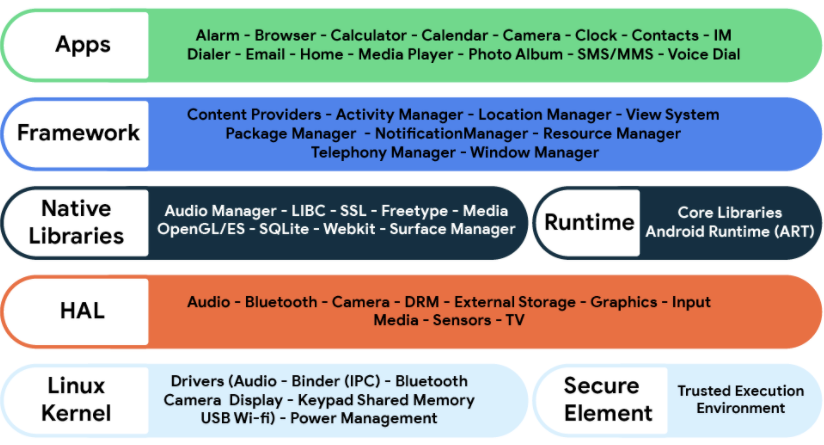
\includegraphics[scale=0.5]{figures/android_os.png}
    \caption{Android platform architecture \protect\cite{5}}
    \label{fig:android_platform_architecture}
\end{figure}

The section below gives a brief description of each major layer of the Android platform architecture mentioned in Fig. \ref{fig:android_platform_architecture}: 

%\subsubsection{Applications}
%Android is an open-source operating system for mobile devices such as mobile phones, tablets, IoT devices and so on. The Android project was initially created by the Open Handset Alliance which includes organizations from various industries such as Google, Vodafone, T-Mobile, LG, Huawei, Asus, Acer, and eBay to give some examples\footnote{\url{http://www.openhandsetalliance.com/oha_members.html}}. The main goal of the Android project is to provide an open software platform accessible for a variety of stakeholders such as developers, engineers, carriers, and device manufacturers to turn their innovative and imaginative ideas into successful real-world products that improve the mobile experience for the end-users. Today, numerous organizations from Open Handset Alliance and also other organizations are supporting and investing in Android and the project is led by Google.

%\subsubsection{Java API Framework}
%The Android operating system's APIs written in Java programming language are provided through this layer. These APIs are the core building blocks for the developers in order to develop Android applications. A couple of noticeable key core building blocks include the following:
\begin{itemize}
\item View System: It provides an extensible set of views for creating user interfaces and user experience.
\item Resource Manager: Providing tools for accessing and managing non-code embedded application resources such as strings, colors, values, layouts, images, etc.
\item Activity Manager: It provides the tools for managing the application lifecycle and navigation back stack.
\item Content Providers: It provides tools for enabling data sharing between different applications.
\item Notification Manager: It provides tools for developers to add the ability of notifications and alerts for Android applications.
\item Location Manager: Provides tools for developers to manage location-related data and location updates.
\end{itemize}
The practices that will be covered in this study mainly occur on this layer because the code is developed and structured in the Java API Framework layer.

%\subsubsection{Native Libraries}
%This layer includes a variety of C/C++ core libraries and Java libraries. The purpose of this layer is to provide support for core features. Important system components of Android, such as HAL (Hardware Abstraction Layer) and ART (Android Runtime) depend heavily on the native libraries that are written on C/C++ programming languages \cite{7}. Some of the important native libraries are Camera, Media, OpenGL, SQLite, WebKit, SurfaceManager, etc.

%\subsubsection{Android Runtime}
%Android Runtime(ART) is a runtime environment for applications that run on the Android operating system. With the launch of Android Version 5.0 or in other words, API level 21, the Dalvik virtual machine was replaced with Android Runtime. Since then, every application started running on its own process along with its own instance of ART \cite{7}.

%\subsubsection{Hardware Abstraction Layer}
%Hardware Abstraction Layer (HAL) is responsible for providing the device hardware features to the Java API Framework layer through interfaces \cite{7}. In other words, it enables the communication between the device hardware and framework. The hardware includes important device features such as Bluetooth, camera, and sensors.

%\subsubsection{Linux Kernel}
%The very core of the Android platform is the Linux Kernel and the base infrastructure of the Android heavily depends on the Linux. Using Linux comes with some advantages. Firstly, using a well-known kernel enables device providers to work on a platform that they already recognize, and second Android benefits from the Linux system and kernel security \cite{7}. This layer also provides all the hardware drivers for camera, display, etc., and handles battery management and other system-related properties.

\subsection{Fundamentals of Android Applications}
\subsubsection{Maintainability}
\textbf{\textit{"Good programmers write code that humans can understand." - Martin Fowler}} \cite{21}

A few decades ago programmers were using low-level programming languages that are working close to computer CPUs. These programming languages were designed to be understood by computers, not humans because computers lacked proper hardware, resources, and speed. Priorities back then were different. The computer programs had to be fast and less memory consuming. However, this situation has changed. Today computers are much stronger and software systems are more complex. However this situation also brought some difficulties to software development. Especially when developing large-enterprise software products, not considering how to overcome these difficulties may cause significant failures. In this context,  this new reality brought new standards to software development. New programming paradigms were born and the priorities have altered \cite{12}.

When the priorities of modern software development are analyzed today, the maintainability of software systems emerges as one of the most critical ones \cite{53}. Maintainability is how well a software system is understandable, repairable, and extendable. In other words, it is a characteristic of software that provides insights into how easily a software system can be maintained \cite{54}. Software systems are born, they live, they change, and eventually, they die. During their lifetime, new features are added, some features are removed, bugs are fixed, and often their development team changes. Usually, there is always a time gap between these changes. Developers should be able to understand the systems easily even months after. Besides, changes to the code base should be able to be done with ease without breaking the other parts of the software system. Ignoring all these might cause companies a significant amount of time and money. Developing maintainable software systems is the way to tackle such issues \cite{50}. In his famous book "Clean Code", Robert C. Martin explains how a top-rated company in the late 80s was wiped out from the business due to the lack of maintainability and poorly managed code organization \cite{11}. When the release cycles of their product extended due to the unorganized code base of their product, they were not able to fix bugs, prevent crashes, and add new features. Eventually, they had to withdraw their product from the market and went out of business. Lousy code and, consequently, lack of maintainability was the reason for this company to go out of the business. Considering the changes in software development since the 80s, this example might sound outdated. However, this real-life incident clearly shows how vital maintainability is to software systems and what fatal consequences it can cause if ignored. 

The importance of maintainability for software systems can also easily be seen when looking at its effect on the software development lifecycle and software development costs. A study has shown that the relative expense for maintaining software and dealing with its development speaks to over 90\% of its absolute expense \cite{4}. The maintenance period for a software system starts as soon as the system is developed. Thus, maintainability becomes a vital aspect for applying new customer needs, adding/removing new features, adapting to the environmental changes \cite{23}. Reports indicate that maintenance cost is 75\% of the total project cost, and the cost for maintaining source code is ten times bigger than developing the source code \cite{22}. The importance of maintainability for software systems is obvious. Also, considering the fast software development lifecycle of mobile applications, the importance of maintainability becomes even more apparent for mobile applications. Facebook's Android application is a good example of this situation\footnote{\url{https://www.apk4fun.com/history/2430/}}. In principle, mobile apps with high maintainability are easier to publish, update and provide high-quality features with less effort. That's why maintenance is considered one of the most important activities for mobile applications \cite{53}.


\subsubsection{SOLID Principles}
\label{section:SOLID}
SOLID stands for five principles \cite{26}. Following are the brief descriptions of each principle:
\begin{itemize}
    \item \textbf{The Single Responsibility Principle:} A class should have only one reason to chance.
    \item \textbf{The Open/Close Principle:} A module should be open for extension but closed for modification
    \item \textbf{The Liskov Substitution Principle:} Subclasses should be substitutable for their base classes.
    \item \textbf{The Interface Segregation Principles:} Many client specific interfaces are better than one general purpose interface 
    \item \textbf{The Dependency Inversion Principle:} Depend upon Abstractions. Do not depend upon concretions
\end{itemize}

The SOLID Design Principles are object-oriented design guidelines to satisfy software quality attributes such as understandability, modifiability, maintainability and testability. The steps to be taken to increase the maintainability of the software systems can be taken at the design stage. The SOLID Principles are very efficient when it comes to solving such design issues and increasing maintainability of software systems.  Not following SOLID principles may lead to serious maintainability problems in the software development lifecycle, such as tight coupling, code duplication, and bug fixing \cite{55}.

\subsubsection{Separation of Concerns}
Software systems have many complex concerns such as persistence, real-time constraints, concurrency, visualization, location control \cite{27}. Software engineering, first of all, aims to increase software quality, lower the expenses of software production, and assist maintenance and development \cite{28}. That is where "Separation of Concerns" (SoC) emerges as a solution. In the context of software engineering, SoC is a software design principle for separating a software system into discrete modules that each module addresses a single concern. A good application of SoC to a software system provides benefits such as increasing maintainability, reducing complexity. The borders for different concerns might differ from a software system to another. Concerns depend on the requirements of a software system and the forms of decomposition and composition. 

Android applications have different concerns such as sustain limited resource availability on mobile devices, user interface responsiveness,  interactions between application components,  network connectivity, local data storage, business domain-specific issues, frequent Android platform-level changes and so on. While dealing with these concerns developers spend a considerable amount thereby they are diverted from their main goal of building production-quality Android applications. Eliminating this complexity can be achieved through focusing on the separation of concerns and abstracting away different concerns from each other. Such a goal can be achieved by applying proper software architecture, e.g. "Clean Architecture" \cite{56}.

\subsubsection{Software Architecture}
In the Android world, the term "content provider" refers to the component that is designed to manage a mutual application data set that can be stored via a file system or a local database (e.g. SQLite) or any other kind of persistent storage. Content providers define, manage, and supply inter-application data sets. Android applications can provide content providers for other Android applications and through the content providers, any other Android application that has the necessary permissions can query the content provider to read and write data within its permissions. From the Android system perspective, a content provider can be considered as an entry point into an Android application in order to issue named data sets identified by a URI scheme. A solid example to a content provider can be given as the content provider that the Android system provides for the purpose of managing the contact information of the user between multiple apps \footnote{\url{https://developer.android.com/guide/topics/providers/content-provider-basics}}.



%\subsubsection{Activity}
%\textbf{\textit{"Good programmers write code that humans can understand." - Martin Fowler}} \cite{21}

A few decades ago programmers were using low-level programming languages that are working close to computer CPUs. These programming languages were designed to be understood by computers, not humans because computers lacked proper hardware, resources, and speed. Priorities back then were different. The computer programs had to be fast and less memory consuming. However, this situation has changed. Today computers are much stronger and software systems are more complex. However this situation also brought some difficulties to software development. Especially when developing large-enterprise software products, not considering how to overcome these difficulties may cause significant failures. In this context,  this new reality brought new standards to software development. New programming paradigms were born and the priorities have altered \cite{12}.

When the priorities of modern software development are analyzed today, the maintainability of software systems emerges as one of the most critical ones \cite{53}. Maintainability is how well a software system is understandable, repairable, and extendable. In other words, it is a characteristic of software that provides insights into how easily a software system can be maintained \cite{54}. Software systems are born, they live, they change, and eventually, they die. During their lifetime, new features are added, some features are removed, bugs are fixed, and often their development team changes. Usually, there is always a time gap between these changes. Developers should be able to understand the systems easily even months after. Besides, changes to the code base should be able to be done with ease without breaking the other parts of the software system. Ignoring all these might cause companies a significant amount of time and money. Developing maintainable software systems is the way to tackle such issues \cite{50}. In his famous book "Clean Code", Robert C. Martin explains how a top-rated company in the late 80s was wiped out from the business due to the lack of maintainability and poorly managed code organization \cite{11}. When the release cycles of their product extended due to the unorganized code base of their product, they were not able to fix bugs, prevent crashes, and add new features. Eventually, they had to withdraw their product from the market and went out of business. Lousy code and, consequently, lack of maintainability was the reason for this company to go out of the business. Considering the changes in software development since the 80s, this example might sound outdated. However, this real-life incident clearly shows how vital maintainability is to software systems and what fatal consequences it can cause if ignored. 

The importance of maintainability for software systems can also easily be seen when looking at its effect on the software development lifecycle and software development costs. A study has shown that the relative expense for maintaining software and dealing with its development speaks to over 90\% of its absolute expense \cite{4}. The maintenance period for a software system starts as soon as the system is developed. Thus, maintainability becomes a vital aspect for applying new customer needs, adding/removing new features, adapting to the environmental changes \cite{23}. Reports indicate that maintenance cost is 75\% of the total project cost, and the cost for maintaining source code is ten times bigger than developing the source code \cite{22}. The importance of maintainability for software systems is obvious. Also, considering the fast software development lifecycle of mobile applications, the importance of maintainability becomes even more apparent for mobile applications. Facebook's Android application is a good example of this situation\footnote{\url{https://www.apk4fun.com/history/2430/}}. In principle, mobile apps with high maintainability are easier to publish, update and provide high-quality features with less effort. That's why maintenance is considered one of the most important activities for mobile applications \cite{53}.


%\subsubsection{Fragment}
%SOLID stands for five principles \cite{26}. Following are the brief descriptions of each principle:
\begin{itemize}
    \item \textbf{The Single Responsibility Principle:} A class should have only one reason to chance.
    \item \textbf{The Open/Close Principle:} A module should be open for extension but closed for modification
    \item \textbf{The Liskov Substitution Principle:} Subclasses should be substitutable for their base classes.
    \item \textbf{The Interface Segregation Principles:} Many client specific interfaces are better than one general purpose interface 
    \item \textbf{The Dependency Inversion Principle:} Depend upon Abstractions. Do not depend upon concretions
\end{itemize}

The SOLID Design Principles are object-oriented design guidelines to satisfy software quality attributes such as understandability, modifiability, maintainability and testability. The steps to be taken to increase the maintainability of the software systems can be taken at the design stage. The SOLID Principles are very efficient when it comes to solving such design issues and increasing maintainability of software systems.  Not following SOLID principles may lead to serious maintainability problems in the software development lifecycle, such as tight coupling, code duplication, and bug fixing \cite{55}.

%\subsubsection{Service}
%Software systems have many complex concerns such as persistence, real-time constraints, concurrency, visualization, location control \cite{27}. Software engineering, first of all, aims to increase software quality, lower the expenses of software production, and assist maintenance and development \cite{28}. That is where "Separation of Concerns" (SoC) emerges as a solution. In the context of software engineering, SoC is a software design principle for separating a software system into discrete modules that each module addresses a single concern. A good application of SoC to a software system provides benefits such as increasing maintainability, reducing complexity. The borders for different concerns might differ from a software system to another. Concerns depend on the requirements of a software system and the forms of decomposition and composition. 

Android applications have different concerns such as sustain limited resource availability on mobile devices, user interface responsiveness,  interactions between application components,  network connectivity, local data storage, business domain-specific issues, frequent Android platform-level changes and so on. While dealing with these concerns developers spend a considerable amount thereby they are diverted from their main goal of building production-quality Android applications. Eliminating this complexity can be achieved through focusing on the separation of concerns and abstracting away different concerns from each other. Such a goal can be achieved by applying proper software architecture, e.g. "Clean Architecture" \cite{56}.

%\subsubsection{Content Providers}
%In the Android world, the term "content provider" refers to the component that is designed to manage a mutual application data set that can be stored via a file system or a local database (e.g. SQLite) or any other kind of persistent storage. Content providers define, manage, and supply inter-application data sets. Android applications can provide content providers for other Android applications and through the content providers, any other Android application that has the necessary permissions can query the content provider to read and write data within its permissions. From the Android system perspective, a content provider can be considered as an entry point into an Android application in order to issue named data sets identified by a URI scheme. A solid example to a content provider can be given as the content provider that the Android system provides for the purpose of managing the contact information of the user between multiple apps \footnote{\url{https://developer.android.com/guide/topics/providers/content-provider-basics}}.



%\subsubsection{Broadcast Receivers}
%The term "broadcast receiver" refers to the Android system component that enables the system to distribute events that happen outside of the normal application flow to the Android applications. Just like the other main Android application components that were mentioned previously, broadcast receivers are also entry points to the Android applications. As a result of that, the Android system can deliver broadcasts to Android applications regardless if the application is running or not. Broadcast in Android tends to originate from the Android system itself. Low battery notification, captured screen notification, and the screen on/of indicators can be given as examples to the Android system broadcasts. However, Android applications can also initiate broadcasts. Broadcast receivers do not involve displaying a user interface but they have the ability to create notifications in the status bar in order to alert users. Android Software Development Kit provides the "BroadcastReceiver" class and each broadcast receiver must be implemented as a subclass of this provided class in Android applications \footnote{\url{https://developer.android.com/reference/android/content/BroadcastReceiver}}.

\subsection{Maintainability}
\textbf{\textit{"Good programmers write code that humans can understand." - Martin Fowler}} \cite{21}

In ancient times, when computers were big, heavy, and slow, programmers were limited to use low-level programming languages that are working close to computer CPUs. These were imperative programming languages, and the programs written in these programming languages were following the procedural programming paradigm. Although that approach worked fine, the biggest problem was that these programming languages were designed to be understood by computers, not humans. The main reason for this situation was that, back in that time, computers lacked proper hardware, resources, and speed. Consequently, the priorities back then were different. The computer programs had to be fast and less memory consuming. However, this situation has changed in the current day. Even a low-quality mobile device is much stronger and smarter than the computers that people were using a couple of decades ago, and software systems became complex. Although this change brought a positive impact on the end-user side as it also brought more functionality and ease, the impact it brought the software development side is complexity. Especially when developing large-enterprise software products, ignoring that fact and not considering how to overcome this complexity may cause significant failures. In this context, new programming languages and paradigms were born, the priorities have altered, and this new reality brought different challenges and new quality standards to software development \cite{12}.

When the priorities of modern software development are analyzed today, the maintainability of software systems emerges as one of the most critical priorities, perhaps even the most important. According to the IEEE Standard Glossary of Software Engineering Terminology, the term "maintainability" is the ease with which a system or component can be modified for use in applications or environments other than those for which it was specifically designed \cite{20}. In the context of software engineering, maintainability means how well a software system is understandable, repairable, and extendable. Maintenance is one of the most important parts of the software development life cycle because the time spent on maintaining software systems requires more time and resources than the rest of the process. The relative expense for maintaining software and dealing with its development speaks to over 90\% of its absolute expense \cite{4}. The level of maintainability that a software system depends on several different factors. Overall, a software system can be considered maintainable if it is simple to grasp how it works and what it does, and making changes such as adding new features and fixing bugs is easy. Besides, maintainability is directly related to well-known software engineering concepts such as coupling, complexity and cohesion. Knowing the relationship between these concepts and maintainability is also essential in measuring maintainability, which is one of the topics of this study. Previous studies have proved this relationship. The inverse ratio between complexity and maintainability was mentioned in Saifan and Rabadi (2017) on measuring maintainability in Android applications \cite{34}. Also, the inverse relationship between coupling and maintainability and the correlation between cohesion and maintainability are discussed in detail in Barak et al., (2012) on maintainability metrics in open-source software \cite{33}.

Considering the life cycle of software systems might help to understand the importance of maintainability. Software systems are born, they live, they change, and eventually, they die. However, their lifetime is generally long, and during their lifetime, new features are added, some features are removed, bugs are fixed, and often their development team changes. Usually, there is always a time gap between these changes. In other words, developers might need to make a change to the software system, which they worked in weeks or months before. In such cases, developers should be able to understand the systems easily even months after. Besides, changes to the code base should be able to be done with ease without breaking the other parts of the software system. Also, when a new developer joins the development team, onboarding should be smooth, and the new developer should be able to understand the purpose of the software system easily. Ignoring all these might cause companies a significant amount of time and money. That is what makes maintainability that important. Developing maintainable software systems is the way to tackle such issues.

The importance of maintainability for software systems can also easily be seen when looking at its role in the software development lifecycle and its effect on software development costs. The maintenance period for a software system starts as soon as the system is developed. Thus, maintainability becomes a vital aspect for applying new customer needs, adding/removing new features, adapting to the environmental changes \cite{23}. The time that has to be spent on the maintenance of complex software products is comparatively more extended than the rest of the software development lifecycle processes. Reports indicate that the amount of effort spent on software maintenance is between 65\% and 75\% of the total amount of effort \cite{13}. Also, another report points out that maintenance cost is 75\% of the total project cost, and the cost for maintaining source code is ten times bigger than developing the source code \cite{22}. In his famous book "Clean Code", Robert C. Martin explains how a top-rated company in the late 80s was wiped out from the business due to the lack of maintainability and poorly managed code organization. When the release cycles of their prominent product extended, due to the unorganized code base of their product, they were not able to fix bugs, prevent crashes, and add new features. Eventually, they had to withdraw their promising product from the market and went out of the business. Lousy code and consequently, maintainability was the reason for this company to go out of the business \cite{11}. This real-life example clearly shows how vital maintainability is to software systems and what fatal consequences it can cause if ignored.

The importance of the maintainability for software systems is evident and this situation is no different for Android Applications. In fact, the importance of maintainability for Android applications is even higher since Android applications have a very active software development life cycle. Given that the growing user demands and business needs making the Android applications more and more complex and Android applications having frequent update rates, it is not hard to see how important the maintainability is for Android application development. This situation is one of the main sources of motivation for this study. 

 In addition to that, in the context of Android, when the main challenges mentioned in this study are evaluated together, the importance of maintainability as a non-functional requirement becomes even more evident for Android application development because the high level of maintainability is the way to overcome the challenges and complexities mentioned in this study while developing Android applications. In consequence, the question is how to achieve the goal of developing Android applications with high maintainability. From the software development point of view, the Android platform does not have strict rules on how the applications are developed. Developing maintainable applications is not an obligation. However, developing Android applications with high maintainability is a need to solve the difficulties mentioned in this study in a timely and cost-efficient manner, facilitate the development processes for the Android developers, and increase the quality of the Android applications. The methods to be followed and the technologies to be used in Android applications for meeting these requirements constantly evolve, and the topic is still controversial among the Android community. Different solutions have been proposed and tried since the birth of the platform. However, the unchanged reality is that the most important criteria for building reliable software systems in a timely and cost-efficient manner is maintainability and of course, this reality is not different for Android applications. 

\subsection{SOLID Principles}
\label{section:SOLID}
In the previous section, the importance of maintainability and maintenance of software systems were explained. The steps to be taken to increase the maintainability of the software systems can be taken at the design stage. Thus maintenance costs of software systems can be minimized. To that aim applying some techniques and principles is essential when developing software systems. The SOLID Principles are very efficient when it comes to solving such design issues and increasing maintainability of software systems. SOLID stands for five principles, namely Single responsibilities principle, Open close principle, Liskov substitution principle, Interface segregation principle, and Dependency inversion principle. Application of SOLID principles when developing software systems via object-oriented programming facilitates improving critical factors such as maintainability, extendability, readability, and reducing code complexity and tight coupling, increasing cohesion \cite{26}. Recalling from the previous sections, factors such as maintainability, extendability, readability, increasing cohesion and reducing code complexity and tight coupling are closely related to the challenges that are faced when developing Android applications. Thus it is wise to use programming techniques that can ensure the application of SOLID principles when developing Android applications. A detailed description of the SOLID principles is beyond the scope of this study. However, briefly summarizing each principle as below will be enough to remind the principles given that the readers of this study are already aware of them. Following are the brief descriptions of each principle \cite{26}:
\begin{itemize}
    \item \textbf{The Single Responsibility Principle:} A class should have only one reason to chance.
    \item \textbf{The Open/Close Principle:} A module should be open for extension but closed for modification
    \item \textbf{The Liskov Substitution Principle:} Subclasses should be substitutable for their base classes.
    \item \textbf{The Interface Segregation Principles:} Many client specific interfaces are better than one general purpose interface 
    \item \textbf{The Dependency Inversion Principle:} Depend upon Abstractions. Do not depend upon concretions
\end{itemize}
Not following SOLID principles may lead to serious maintainability problems in the software development lifecycle, such as tight coupling, code duplication, and bug fixing. Application of SOLID design principles when developing software systems helps to achieve essential quality factors such as understandability, flexibility, maintainability, and testability \cite{26}.

\subsection{Separation of Concerns}
Today, the complexity of software applications is quite high, and it still is increasing. Today's software systems have many complex concerns such as persistence, real-time constraints, concurrency, visualization, location control \cite{27}. Software engineering, first of all, aims to increase software quality, lower the expenses of software production, and assist maintenance and development. In achieving these aims, software engineers are continuously on the lookout for developing technologies and approaches that increase maintainability, decrease software complexity, enhance understandability, support reuse, and boost development. That is where "Separation of Concerns" (SoC) emerges as a solution. 

In the context of software engineering, SoC is a software design principle for separating a software system into discrete modules that each module addresses a single concern. A good application of SoC to a software system provides benefits such as increasing maintainability, reducing complexity. The borders for different concerns might differ from a software system to another. Concerns depend on the requirements of a software system and the forms of decomposition and composition \cite{28}. 

In the context of Android, the importance of SoC is even more apparent. Android applications have different concerns with clearly drawn borders. Such concerns can be named as visualization and presentation of data, business logic, networking, persistence, location services. Depending on the requirements of an Android application, there might be other concerns as well. In light of the information above, it is vital to identify these concerns before Android applications are developed, and during the development phase, to use techniques that can apply SoC well.

\subsection{Software Architecture}
\textbf{\textit{“Good architecture makes the system easy to understand, easy to develop, easy to maintain, and easy to deploy. The ultimate goal is to minimize the lifetime cost of the system and to maximize programmer productivity.” - Robert C. Martin}} \cite{10}

The previous section explained that software systems are not static environments. They grow, change, and get updated based on the new requirements. During this change, new additions are made in forms of components, methods, modules. As the system grows, the interactions between these different system elements also get more complicated and all together lead to complexity in software systems. In order to be able to develop reliable software systems that can overcome this complexity, programmers must implement software systems in a generalized fashion. Software systems that are written in such fashion can be considered reliably usable, maintainable, testable, and extendable \cite{15}. 

At that stage, the question is, what would be the so-called generalized fashion from the software engineering perspective. A couple of decades ago, software engineers and researchers started paying more attention to this topic and started studies to find an answer to this question. These studies were intended to find solutions for the problems emerging while developing large scale software systems. The focus area of these studies started as software design and eventually evolved into software architecture \cite{24}. The answer to the above question today is software architecture. Martin Fowler defines the meaning of the architecture in the software industry as "the shared understanding that the expert developers have of the system design" \cite{16}. Technically speaking, software architecture is "the set of significant decisions about the organization of a software system, the selection of structural elements and their interfaces by which the system is composed, together with their behavior as specified in the collaborations among those elements, the composition of these elements into progressively larger subsystems, and the architectural style that guides this organization -- these elements and their interfaces, their collaborations, and their composition" \cite{17}. 

Good architecture facilitates the satisfaction of requirements for software systems as well as providing better performance and more reliability. Today the impact of software architecture on the success of software systems is quite high. Selecting the right architecture for a software system is a critical success factor for system design and development. As Brian Foote quotes, "if you think good architecture is expensive, try bad architecture"\cite{10}. Also, software architecture has a central role between software implementation and requirements. The role of software architecture in software development can be elaborated under the six major aspects. Those aspects can be listed as follows \cite{25}:
\begin{itemize}
    \item \textbf{Understanding:} Good architectural design simplifies the understanding of systems, in the context of what the system does and how it does as well as facilitating the understanding of the systems’ high-level design. Thus good architecture improves the readability of software systems.
    \item \textbf{Reuse:} Good software architecture facilitates and increases the code reuse between the components.
    \item \textbf{Construction:} Software architecture provides a good outline of the software system in the form of layers and abstractions. The outline describes the components of the system and dependencies between those components.
    \item \textbf{Evolution:} Software architecture can point out the dimensions which a software system might evolve to. Therefore software architecture helps software teams to understand the consequences of changes more accurately. Moreover, software architecture describes how the concerns of the software systems are separated and it determines the boundaries of interactions between those concerns. 
    \item \textbf{Analysis:} A well-applied software architecture enables analyzing the system consistency, compliance with restrictions imposed by the architecture, and compliance with the quality attributes.
    \item \textbf{Management:} Assessment of software architecture facilitates understanding of risks, requirements, and implementation strategies.
\end{itemize}
When contemplating the importance of software architecture for Android application development, of course, there is no difference. When the fast update rate of Android applications, frequent requirement changes of Android projects, and the complex issues and restrictions that arise from the nature of Android are taken into consideration, the significance of software architecture selection when developing Android applications becomes even more prominent. However, this area has been problematic for Android application development and Android developers from the beginning.

During the early days of Android development, Android developers tended to use "god activities". God activities were activities where developers place all kinds of code including user interface, presentation logic, business logic, and so on. This unstructured way of a software development approach that does not follow any architectural or design pattern is called "anti-pattern". Back then, Android applications were relatively smaller and less complex. Ever since the Android applications started becoming more and more complex these god activities became a black hole for Android developers because they were hard to read, understand, test, and maintain. Android developers were quick to recognize these problems and needs and had no trouble finding solutions on how to develop Android applications in a more organized way. In order to solve this god activity and such an anti-pattern problem and improve the maintainability of Android applications, Android developers started applying well-known and widely used architectural and design patterns in GUI-heavy applications to Android application development \cite{19}. With improvements and advancements in hardware and software and growing demand for the user and business needs, the requirement for developing organized and maintainable Android applications has had a great extent \cite{18}.

Today, though the use of architectural patterns and design patterns in Android application development does not seem to be a requirement, it is actually of a de-facto must. Developing an Android application without applying an architectural pattern would be a bad decision because complex applications that do not follow any architectural pattern are expected to end up with serious maintainability issues. Also, surviving in such a competitive market is heavily dependent on developing a well-architected Android application that has a high level of maintainability. While developing Android applications, the expectation in terms of software architecture is to apply the SOLID principles and separation of concerns in a healthy way and to have high maintainability. On the other hand, there is no fixed solution for that problem that Android demands from developers to meet its applications and there are a variety of options. So, the right way to architect Android apps still remains in discussion with clashing standpoints which are generally affected by technological hypes \cite{14}.

Importance of the software architecture in terms of software systems and especially Android applications was explained above. At this point, it will be of utmost importance to emphasize the relationship between architectural choice and maintainability, as the main subject of the study is the improvement of the maintainability of Android applications. Can it be claimed that maintainability is the most crucial quality requirement when developing Android applications when it comes to architectural selection? With many options available for architecting Android applications, what is the top quality requirement that an Android application architecture should provide in order to overcome the complexities? As this study has emphasized continuously since the beginning, the answer to these questions is maintainability. A related study had conducted a questionnaire between Android practitioners and researched other related academic papers and results had revealed that the top quality requirement for architecting Android applications is maintainability \cite{14}.
\begin{figure}[ht!]
    \centering
    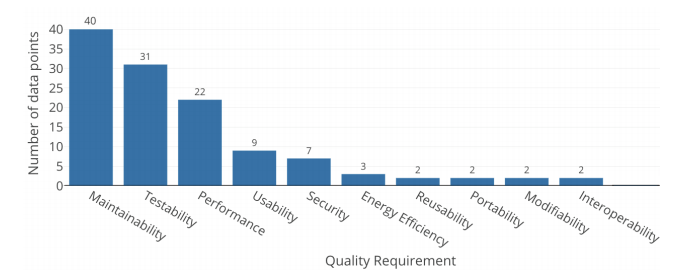
\includegraphics[scale=0.6]{figures/quality_req.png}
    \caption{Quality requirement rankings for architecting Android apps \protect\cite{14}}
    \label{fig:arch_quality_req_ranking}
\end{figure}

It is proven that maintainability and selection of architectural patterns when developing Android applications are directly in correlation. In addition, it can be said that other quality requirements presented in the figure above, apart from maintainability, directly affect maintainability itself. In particular, quality requirements such as modifiability, testability and reusability will increase as the maintainability increases, or vice versa. As a consequence, the impact of the architectural pattern on the maintainability of Android applications is one of the top aspects that should be considered when making the decision of the architectural pattern before starting the development of a new Android application.

\subsection{Literature Review}
\label{section:2.7}
In this section, the outcomes obtained from examining the academic studies on Android application development are presented. Considering the tight relationship between the topic and industry, a Systematic Literature Review (SLR) was not adequate for finding relevant resources of data for the study. Hence, a Multivocal Literature Review (MLR) was conducted. As a type of SLR, MLR is collecting grey literature as well alongside formal literature \cite{40}. MLR considers resources like blogs, white papers, articles, academic literature and allows gathering information from academics, developers, practitioners, and independent researchers \cite{41}. For a topic closely related to the industrial trends, adding grey literature next to the white literature as a part of the literature review was crucial. Because the most up-to-date resources are the grey literature resources in the Android environment and to compare the white literature's situation to the latest industrial trends of the Android application development, grey literature is definitely needed. Regardless of the direct relevance of the studies to maintainability, the following research query has been used to determine all the studies related to Android application development published in the last five years. Among the determined studies, those related to maintainability have been examined in more detail. 
\begin{figure}[ht!]
    \centering
    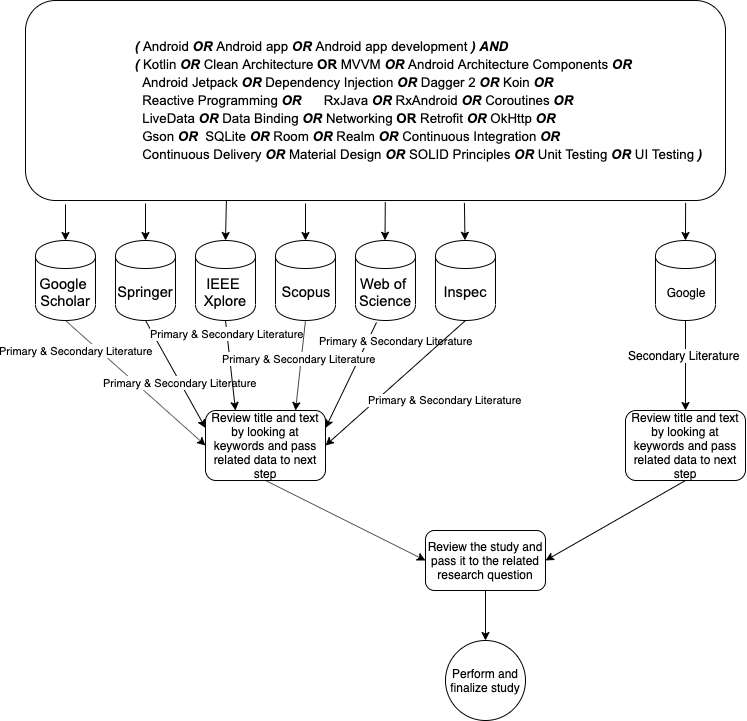
\includegraphics[scale=0.4]{figures/research_query.png}
    \caption{Search process visualization}
    \label{fig:lit_review_research_query}
\end{figure}

As a result of the executed research query above, more than forty seven papers were found and reviewed. Grey literature results are not included in these numbers. The found and reviewed grey literature results were only used to compare the academic literature and industry's situation and interpret the situation. Also, the reviewed grey literature was cited in this study. For the purpose of obtaining more successful findings, the search query was separated into six parts, each of them individually focusing on a single topic. The literature found as a result of this query was read thoroughly. Finally, inclusion and exclusion criteria were applied to the primary studies to have suitable literature only. As soon as the early research outcomes were collected, chasing the inclusion and exclusion criteria shown in Figure 6, the unrelated material was filtered out. Also, the studies conducted before 2015 are excluded from the query results to prevent any possible up-to-dateness issues.
\begin{figure}[ht!]
    \centering
    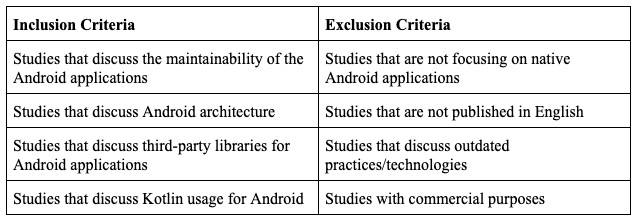
\includegraphics[scale=0.6]{figures/research_query_criteria.png}
    \caption{Inclusion and exclusion criteria}
    \label{fig:lit_review_research_query_criteria}
\end{figure}

These more than forty academic studies examined on Android application development can be grouped according to their topic titles as follows.
\begin{itemize}
    \item 4 studies bachelor theses regarding Android application development.
    \item 5 papers were related to 3rd party Android libraries.
    \item 5 papers were related to Kotlin programming language usage for Android.
    \item 5 papers were related to maintainability of the Android applications.
    \item 12 papers were related to Android app architecture.
    \item 16 papers were related to Android application development but not directly related to the topic that this study covers.
\end{itemize}

In addition to the papers mentioned above, 15 other papers are reviewed to get a better understanding of the studies conducted regarding software maintainability, metrics that can be used to measure software maintainability, general software engineering principles such as separation of concerns, and SOLID. These articles and books have been cited in various parts of this study.

Among these more than forty academic studies on Android application development that are reviewed as a part of this study, the studies on Android application architecture and maintainability draw attention. Studies conducted on these two subjects account for more than one-third of the total studies examined. Based on these numbers, it can be said that the Android application architecture and the importance of maintainability are recognized by the researchers working in the Android field. As stated in the 2.3 and 2.6 sections of this study, the importance of application architecture and maintainability in the context of Android application development processes is supported by the above numbers and academic studies included in these numbers. In most of these studies, it is noteworthy that comparisons of Android application architectures in terms of performance, maintainability, and testability are common. As mentioned in previous chapters, considering the impact of software architecture on maintainability and the importance of maintainability in software development processes, it is not surprising that many academic studies have focused on architecture and maintainability. Various studies on the maintainability of Android applications draw attention. For example, Hugo Källstrom conducted a study on a similar topic in which he implemented three different software architectures and evaluated the maintainability based on these architectures \cite{18}. Also, Prabowo et al. have a research on the maintainability of Android applications which they compared MVP and anti-pattern approaches \cite{19}. Apart from these works, the work of Verdecchia et al. (2019) on architectural choices in Android applications is a worth reading work on both architecture and maintainability topics \cite{14}. These studies regarding the architecture and maintainability in Android application development stand out as resources worth examining. There are also some other studies that are cited in the paper, they are worth reading too. On the other hand, there are some significant issues with most academic studies regarding the topic. 

First of all, it is noteworthy that academic studies in this field are inadequate. Even as a result of a comprehensive literature review that included the grey literature, around fifty studies were reached, and this number is the total number of studies on Android development. The number of studies on the maintainability of Android applications is slightly less than one-third of this total number. As explained in the previous sections, considering the importance of maintainability in Android application development, it will be seen that the number of studies in this field is insufficient. 

In addition to this quantitative problem, it is seen that there are some qualitative problems among the existing academic studies as well. As a result of the research among academic studies regarding Android application development, the conclusion is that the inadequacy of the formal resources in terms of up-to-dateness constitutes a major issue. Considering the dates of the studies and the continuous and rapid development of the Android world and the changing trends, this result is not unexpected but still points to an issue. That situation creates one of this study's motivations, which is closing this gap between industry and academia. When the literature review results are evaluated in terms of maintainability, which is the main element of this study, some significant issues are observed. 

When the studies on the maintainability of Android applications are examined, we see that many studies approach maintainability in terms of software architecture. As mentioned earlier in this study, it can be said that this result is not a surprise, considering that software architecture is one of the most significant factors in the impact on maintainability. Both academic resources and information gathered from the industry indicate that, when it comes to building Android applications with high maintainability, the architectural choices are shaped around the same main architectural and design patterns. Those can be named as MVC, MVP, MVVM and Clean Architecture. However, When the existing studies are examined, most of the studies cover the basic implementation of these design patterns and comparisons between these design patterns in terms of performance and maintainability. 
\begin{figure}[ht!]
    \centering
    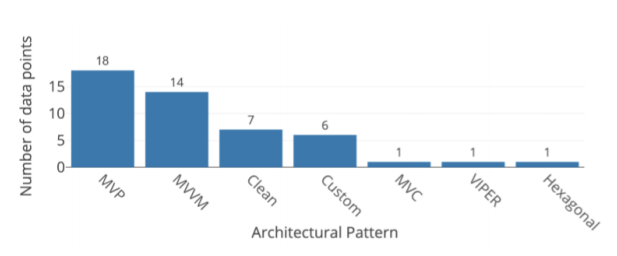
\includegraphics[scale=0.5]{figures/pattern_usage.png}
    \caption{Well-known architectural and design patterns for Android \protect\cite{14}}
    \label{fig:arch_patterns}
\end{figure}

On the other hand, considering the other factors affecting the maintainability of Android applications and some of the outdated techniques and technologies used in the studies mentioned above, it is possible to talk about the insufficiency of these studies on Android application development in the last five years. The systematic review indicates that the lack of detail and outdatedness in these studies is apparent. Another problem that strikes the eye among the academic studies reviewed is that most studies only approach the maintainability of Android applications from an architectural perspective. It is possible that other techniques and technologies can be used to increase the maintainability of Android applications besides architectural patterns. The fact that the studies do not focus on these techniques and technologies can be considered a deficiency of the academic literature regarding this topic.

In addition to the above-mentioned situation, in almost all of the examined academic studies and the reviewed work from the industry, the fact that these design patterns are presentational design patterns and they are not architectural patterns is completely ignored. In other means, the patterns derived from the MV-I concept, such as MVVM, MVP, MVC, are actually designed for how data is managed for display purposes. MV-I design patterns are intended to control the communication between the view layer and the data layer of GUI heavy applications. However, while developing small-sized Android applications, these design patterns can be effective up to a point. Nevertheless, while developing enterprise Android applications that have more sophisticated and complex business logic, it is obvious that these design patterns will be insufficient in scaling the application and solving the maintainability problems we have mentioned. Hence, the visibility of the need for higher-level architecture and other techniques when developing complex Android applications is clear.  Also, considering the study topic's tight relation with the industry, knowing the technologies, techniques, and latest trends used in the industry is also essential for studies on this subject. However, when current studies are examined, it will be seen that there are problems related to these situations.

The literature review shows that the academia lacks awareness of the industry trends and comprehensive information about techniques and technologies that can be used to develop maintainable Android applications with up-to-date tools. This study aims to fill this gap in the academia by explaining and analyzing one of the top mobile application development companies' methodologies in the region.

\subsection{Summary}
In this section, a set of essential information regarding software engineering and Android platform information was shared, and the motivation of the study was covered. The purpose of sharing fundamental software engineering principles such as maintainability and SOLID principles is to shine a light on the background of this study's problem and facilitate understanding of the problem that this study is trying to solve. Again, with the same purpose, necessary information about the Android platform was also shared. The insights of maintainability issues in software development and the consequences of software development complexity issues were covered and interpreted in general. It was also indicated why the challenges get even more complicated when it comes to Android application development. Lastly, the conducted multivocal systematic review of the existing academic papers was shared and interpreted as part of this study.







